
\documentclass[12pt]{amsart}
\usepackage{geometry} % see geometry.pdf on how to lay out the page. There's lots.
\geometry{a4paper} % or letter or a5paper or ... etc
% \geometry{landscape} % rotated page geometry
\usepackage{graphicx}
% See the ``Article customise'' template for come common customisations
\usepackage{amsmath}
\title{2D Collision-Free Transformation}
\author{Ziqi Wang}
\date{} % delete this line to display the current date
\newcommand{\bt}{\mathbf{t}}
\newcommand{\bn}{\mathbf{n}}
\newcommand{\bq}{\mathbf{q}}
\newcommand{\bp}{\mathbf{p}}
\newcommand{\bc}{\mathbf{c}}
\newcommand{\tq}{\mathbf{\hat{q}}}
\newcommand{\tp}{\mathbf{\hat{p}}}
\newcommand{\barq}{\mathbf{\bar{q}}}
\newcommand{\barp}{\mathbf{\bar{p}}}
%%% BEGIN DOCUMENT
\begin{document}

\maketitle

\section{one is static and one is dynamic}
\begin{figure}[!htbp]
  \centering
    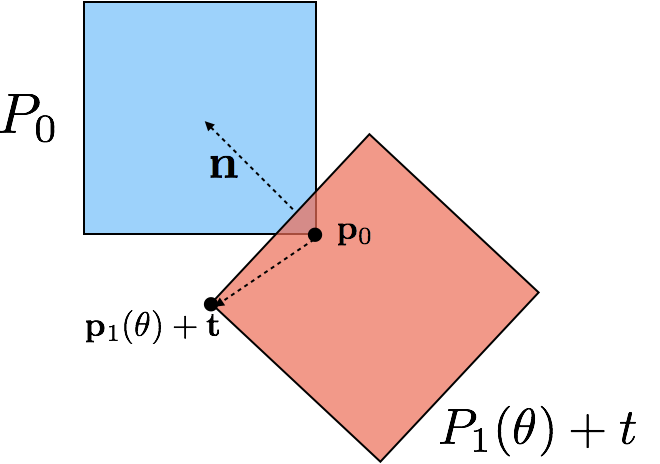
\includegraphics[width=0.6\textwidth]{1fixed1move.png}
      \caption{blue is fixed and red is movable}
\end{figure}
The penetration distance between $P_0$ and $P_1$ in this figure is $\bn^T[\mathbf{p}_1(\theta) + \bt - \mathbf{p}_0]$. Even though for different $\theta, \bt$ there is a different way of choosing $p_0, p_1, \bn$, let us assume that it won't change locally. More specifically:\\
when $|\theta - \theta_0|<\epsilon$, $|\bt - \bt_0|<\epsilon$\\
the penetration distance $d(P_1(\theta, \bt),P_0)$ can be linearize: 
\begin{equation}
	d(P_1(\theta, \bt),P_0) \approx d(P_1(\theta_0, \bt_0),P_0) + \Delta d(P_1(\theta_0, \bt_0),P_0)^T \begin{bmatrix}
		\theta - \theta_0\\
		t^x - t^x_0 \\
		t^y - t^y_0
		\end{bmatrix}
	\end{equation}
Then, using trust region method, the $K$ iteration optimization function is:
\begin{align}
	&\min_{\theta^K, \bt^K} ||d(P_1(\theta^K, \bt^K),P_0)||^2 \\
	\text{subject: } & |\theta^K - \theta^{K-1}| \leq \epsilon^K \\
			       & |\bt^K - \bt^{K-1}| \leq \epsilon^K
\end{align}
With:
\begin{equation}
	d(P_1(\theta^K, \bt^K),P_0) = d(P_1(\theta^{K-1}, \bt^{K-1}),P_0) +  \Delta d(P_1(\theta^{K-1}, \bt^{K-1}),P_0)^T \begin{bmatrix}
		\theta^K - \theta^{K-1}\\
		t_x^K - t_x^{K-1} \\
		t_y^K - t_y^{K-1}
		\end{bmatrix}
	\end{equation}
Specific $d$:
\begin{align}
	d(\theta, \bt)& = \bn^T(\bq(\theta, \bt) - \bp)\\
			   &= \bn^T(R_\theta(\bq -\tq)+\bt +\tq - \bp)\\
			   &= \bn^T(R_\theta\barq+\bt +\bc_0)\\
	d(\theta, \bt) &\approx \bn^T(R_{\theta_0}\barq+\bt_0 +\bc_0) +\bn^T(R'_{\theta_0} \barq (\theta - \theta_0)+(\bt - \bt_0)) \\
			   &= a_0 + \bn^T(R'_{\theta_0} \barq (\theta - \theta_0)+(\bt - \bt_0)) \\
			   &= a_0 + a_1\theta + a_2x + a_3 y
\end{align}
\begin{align}
				a_1 &= \bn^TR'_{\theta_0} \barq \\
				a_2 &= \bn_0 \\
				a_3 &= \bn_1 \\
				a_0 &=  \bn^T(R_{\theta_0}\barq+\bt_0 +\bc_0) -\theta_0\bn^TR'_{\theta_0} \barq - \bn^T\bt_0 \\
				       &= \bn^T(\bq_0 - \bp) - \theta_0\bn^TR'_{\theta_0} \barq - \bn^T\bt_0 \\
				       &= \bn^T(\bq_0 - \bp) - a_1\theta_0 - \bn^T\bt_0
\end{align}

for two moving points:
\\Specific $d$:
\begin{align}
	d(\theta, \bt)& = \bn^T(\bq(\theta^0, \bt^0) - \bp(\theta^1, \bt^1))\\
			   &= \bn^T(R_{\theta^0}(\bq -\tq)+\bt^0 +\tq - R_{\theta^1}(\bp -\tp) - \bt^1 - \tp)\\
	d(\theta, \bt) &\approx \bn^T(\bq_0 - \bp_0) +  \bn^T(R'_{\theta^0_0} \barq(\theta^0 - \theta^0_0) + \bt^0 - \bt^0_0 - R'_{\theta^1_0}(\theta^1 - \theta^1_0) \barp - \bt^1 + \bt^1_0) \\
			   &= a_0 + a_1\theta^0 + a_2x^0 + a_3 y^0 + a_4\theta^1 + a_5x^1 + a_6 y^1
\end{align}
\begin{align}
				a_1 &= \bn^TR'_{\theta^0_0} \barq_0 \\
				a_2 &= \bn_0 \\
				a_3 &= \bn_1 \\
				a_4 &= -\bn^TR'_{\theta^1_0} \barp_0 \\
				a_5 &= -\bn_0 \\
				a_6 &= -\bn_1 \\
				a_0 &=  \bn^T(\bq_0 - \bp_0) - a_1\theta^0_0 - \bn^T \bt^0_0 + a_4 \theta^1_0 + \bn^T \bt^1_0 
\end{align}

\begin{align}
	(\mu \mathbf{a} + (1-\mu) \mathbf{b} - \bq) ^T( \mathbf{a}-  \mathbf{b}) &= 0 \\
	\mu( \mathbf{a} -  \mathbf{b})^T( \mathbf{a} -  \mathbf{b}) + ( \mathbf{b} - \bq)^T( \mathbf{a}-  \mathbf{b}) & = 0 \\
	\mu &= \frac{( \bq - \mathbf{b} )^T( \mathbf{a}-  \mathbf{b})}{( \mathbf{a} -  \mathbf{b})^T( \mathbf{a} -  \mathbf{b})}
\end{align}
\end{document}